\documentclass[a4paper,12pt]{article}
\usepackage{dmasproject}
%Some packages I commonly use.
\usepackage[english]{babel}
\usepackage{lscape}
\usepackage{graphicx}
\usepackage{blindtext}
\usepackage{framed}
\usepackage[normalem]{ulem}
\usepackage{amsmath}
\usepackage{amsthm}
\usepackage{amssymb}
\usepackage{amsfonts}
%\usepackage{algorithm}
%\usepackage[noend]{algpseudocode}
\usepackage{hyperref}
\usepackage{enumerate}
\usepackage[utf8]{inputenc}
\usepackage{fancybox}
\usepackage{tikz}
\usepackage[top=1 in,bottom=1in, left=1 in, right=1 in]{geometry}
\usepackage{clrscode3e}
\usepackage{listings}
\usepackage{xcolor} % for setting colors
\usepackage{cleveref}
\usepackage{lscape}
\usepackage{fancyvrb}
\RecustomVerbatimCommand{\VerbatimInput}{VerbatimInput}%
{fontsize=\footnotesize,
 %
 frame=lines,  % top and bottom rule only
 framesep=2em, % separation between frame and text
 %
 label=\fbox{Output file},
 labelposition=topline,
 %
 commandchars=\|\(\), % escape character and argument delimiters for
                      % commands within the verbatim
 commentchar=*        % comment character
}
% set the default code style
\lstset{
    frame=tb, % draw a frame at the top and bottom of the code block
    tabsize=4, % tab space width
    showstringspaces=false, % don't mark spaces in strings
    numbers=left, % display line numbers on the left
    commentstyle=\color{green}, % comment color
    keywordstyle=\color{blue}, % keyword color
    stringstyle=\color{red} % string color
}

\usetikzlibrary{arrows}
\usetikzlibrary{shapes, snakes}
\tikzset{
	treenode/.style = {align=center, inner sep=0pt, text centered,
		font=\sffamily},
	arn_n/.style = {treenode, circle, white, font=\sffamily\bfseries, draw=black,
		fill=black, text width=1.5em},% arbre rouge noir, noeud noir
	arn_r/.style = {treenode, circle, red, draw=red, 
		text width=1.5em, very thick},% arbre rouge noir, noeud rouge
	arn_x/.style = {treenode, rectangle, white, draw=black, fill=black,
		minimum width=0.1em, minimum height=0.5em, text width=1.5em, very thick},% arbre rouge noir, nil
	arn_reg/.style = {treenode, circle, draw=black,	text width=1.5em, thick},% arbre rouge noir, nil
	empty/.style = {treenode, circle, draw=black,	text width=2em},
	empty_heavy/.style = {treenode, circle, draw=red, text width=2em}
}
%A bunch of definitions that make my life easier
\newcommand{\matlab}{{\sc Matlab} }
\newcommand{\cvec}[1]{{\mathbf #1}}
\newcommand{\rvec}[1]{\vec{\mathbf #1}}
\newcommand{\ihat}{\hat{\textbf{\i}}}
\newcommand{\jhat}{\hat{\textbf{\j}}}
\newcommand{\khat}{\hat{\textbf{k}}}
\newcommand{\minor}{{\rm minor}}
\newcommand{\trace}{{\rm trace}}
\newcommand{\spn}{{\rm Span}}
\newcommand{\rem}{{\rm rem}}
\newcommand{\ran}{{\rm range}}
\newcommand{\range}{{\rm range}}
\newcommand{\mdiv}{{\rm div}}
\newcommand{\proj}{{\rm proj}}
\newcommand{\R}{\mathbb{R}}
\newcommand{\N}{\mathbb{N}}
\newcommand{\Q}{\mathbb{Q}}
\newcommand{\bigo}{\mathcal{O}}
\newcommand{\Z}{\mathbb{Z}}
\newcommand{\<}{\langle}
\renewcommand{\>}{\rangle}
\renewcommand{\emptyset}{\varnothing}
\newcommand{\attn}[1]{\textbf{#1}}
\theoremstyle{definition}
\newtheorem{theorem}{Theorem}
\newtheorem{corollary}{Corollary}
\newtheorem{definition}{Definition}
\newtheorem{example}{Example}
\newtheorem{example_s}{Solved Exercise}
\newtheorem*{note}{Note}
\newtheorem*{solution}{Solution}
\newtheorem{exercise}{Exercise}
\newtheorem*{problem}{Problem}
\newcommand{\bproof}{\bigskip {\bf Proof. }}
\newcommand{\eproof}{\hfill\qedsymbol}
\newcommand{\Disp}{\displaystyle}
\newcommand{\qe}{\hfill\(\bigtriangledown\)}
\setlength{\columnseprule}{1 pt}
% if you need additional LaTeX packages, add them here
\crefname{lstlisting}{listing}{listings}
\Crefname{lstlisting}{Listing}{Listings}
\title{Reconfiguration of Spanning Trees in Networks in the Presence of Node Failure}
% sort your names alphabetically by last name
\author{
  Vladimir Frants,
  Yunhua Zhao
}
\date{\today} % change this accordingly

\begin{document}

\maketitle

\begin{abstract} Logical connectivity in a computer network is usually represented by spanning tree. In the case of failure of one of the nodes of a spanning tree should be reconfigured in a fast and efficient manner with the use of the knowledge of underlying hardware connectivity. In our final project, we implement one of the methods for spanning tree reconfiguration, which addresses the issue of graph fragmentation, the situation when two connected components of the network try to connect avoiding cycles. We implemented the algorithm with the use of python programming languages as a set of nodes that could be run on one or several Linux machines and communicate using TCP/IP protocol.  
\end{abstract}

\section{Introduction}

The connectivity in wide-are network can be represented by a network level abstraction of spanning tree graph. In such a graph vertices represent routers of the network and edges represent communication links between routers. This graph describes a logical connectivity of vertices and edges on top of the physical connectivity of nodes and links. The paper 

The network consists of a set of nodes $\mathcal{V}$ connected by point-to-point links. A graph $\mathcal{G}(\hat{\mathcal{U}}, \hat{\mathcal{E}})$ represents a communication path through a set nodes of the network $\hat{\mathcal{U}}$. Edges $\hat{\mathcal{E}}$ map one-to-one to the existing links. Here $\hat{\mathcal{G}}$ may be viewed as an unrooted spanning tree for users, whereby the user residing in a node $u\in\hat{\mathcal{G}}$ may execute algorithms for traversing a tree $\mathcal{T}_{u}(\mathcal{G})$ with root at $u$ and leaves at nodes $(U-u)$. For instance, the user may be a transport level host in a network and the tree traversal over the edges may allow identification of data routes to the other hosts. $\mathcal{G}$ thus embeds a set of trees $\{\mathcal{T}_{u}(\mathcal{G})\}_{\forall u\in\mathcal{U}}$. 

We assume that the network provides reliable $FIFO$ transmission of messages over a link and that transmission delay over a link is bounded. We also assume that the network diameter $\mathcal{D}$ is finite. 

\section{Problem Motivation}

When a node containing a vertex $u'$ fails (say, due to a crash), a reconfiguration algorithm in the network creates a set of edges to interconnect the various vertices $\in\hat{\mathcal{U}}$ that are adjacent to $u'$. Such an algorithm basically causes recomputing the data paths in $\mathcal{G}$ through the newly created edges. 

A fundamental problem in logical topology re-configurations is handling of \emph{fragmentation} in a graph, whereby two or more subgraphs not connected with one another (or fragments) need to be connected together by creating edges and vertices over appropriate links and nodes respectively in the physical topology to form a composite graph. Typically, the failure of a node containing a vertex fragments the graph at this vertex so that these fragments reconnect with one another circumventing the failed node   \ref{fig:example_graph}. 

\begin{figure}[!h]
    \centering
    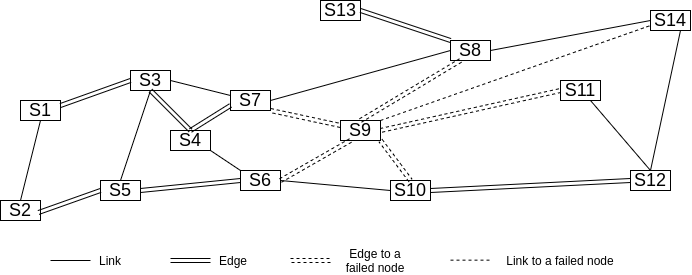
\includegraphics[width=0.85\textwidth]{distributed.png}
    \caption{Network graph}
    \label{fig:basic_octree}
\end{figure}

Prior to failure, node $S_{9}$ had graph edges to its neighbors $S_{6}$, $S_{7}$, $S_{8}$, $S_{10}$ and $S_{11}$. After the failure, the sets of nodes $\{S_{1}, S_{3}, S_{4}, S_{7}\}$, $\{S_{2}, S_{5}, S_{6}\}$, $\{S_{10}, S_{12}\}$, $\{S_{8}, S_{11}\}$ constitute the fragments. 

A fragment is identified by the id of one of its constituent nodes, namely a neighbor of the failed node that has a vertex and detects the failure (e.g. in Figure \ref{fig:example_graph} $\{S_{10}, S_{12}\}$ is identified by the node id of $S_{10}$). The node which detects the failure starts the recnfiguration activity on behalf of its fragment to find physical paths to connect to other fragments. Often, there can be several neighbors of a failed node which may detect the failure and each of these nodes may initiate a reconfiguration activity.

When a set of fragments attempt to connect with one another it is necessary to prevent cycles from being formed in the composite graph as a result of the reconfiguration. Preventing of cycles basically requires the fragments to coordinate with one another in some form. Consider, for instance, two fragments $F_{1}$ and $F_{2}$ attempting reconfiguration. If $F_{1}$ and $F_{2}$ connect independently with each other, the resulting graph can contain cycles. To prevent this, a possibility is for $F_{1}$ and $F_{2}$ to coordinate with each other so that only one them connects to the other. We model this coordination problem as one of resolving contention among the fragments to elect a coordinator which then creates edges to interconnect the various fragments. 

Suppose the fragment $\{S_{10}, S_{12}\}$ becomes the coordinator after contention with other fragments. The nodes $S_{10}$ and $S_{12}$ execute a protocol to create edges between the pairs of nodes (say) $[S_4, S_6]$, $[S_7, S_8]$, $[S_6, S_10]$, and $[S_{11}, S_{12}]$. Thus, there are two basic components of a reconfiguration algorithm, the election and the creation of edges. 

\section{Implementation}

The physical connectivity information is maintained in a node internal table. Consider a node $S$. Let $\{S^{j}\}_{j=1,2,\dots,K}$ be a set of nodes that are neighbors to $S$, i.e., nodes with a link from $S$. Then $\{id(S^{j}), port_{j})\}$ constitutes the physical connectivity table of $S$, where $id(S^{j})$ is the network-wide unique id of $S^{j}$ and $port_{j}$ refers to a node level port (i.e., network interface) through which $S$ is linked to $S^{j}$. The network implements a function \textbf{Port\_To}($S^j$) to extract $port_{j}$ from the table and a function \textbf{Set\_of\_ports} to extract the list of ports to all neighboring nodes. With a unique id for every node in the network, the tables at all nodes specify the physical connectivity in the network. $S$ may execute a separate protocol whereby $S$ can detect the removal of a neighbor (say due to failure) and the addition of a node as a neighbor, and update the table accordingly. 

A function \textbf{Assign\_Edge}($port_j$) is provided that creates a directed edge from $S$ originating through $port_j$ and incident on the neighbor $S_{j}$ so that $S$ becomes adjacent to $S^{j}$ in the graph. A function $\textbf{Get\_Port}$ is also provided that generates a list of port through which $S$ has edges to its adjoining vertices. 



\begin{table}[]
\begin{tabular}{|l|l|}
\hline
\textbf{name} &  \\ \hline
\textbf{my\_id} &  \\ \hline
\textbf{coord\_so\_far} & This is the local view of a node as to which fragment is coordinating. When a node detects the failure of a neighbor and starts a reconfiguration, it sets coord\_so\_far to its own id my\_id \\ \hline 
\textbf{port\_to\_coord} & This is the port in a node through which the fragment identified in coord\_so\_far can be reached. When coord\_so\_far=my\_id the port\_to\_coord is set to NULL \\ \hline
\textbf{status} & This indicates either IDLE or WAIT, meaning respectively that a node is not participating or otherwise in a reconfiguration \\ \hline
\textbf{recd\_reply} &  This gives information about a port as to whether a response has been received through that port indicating completion of the reconfiguration activity in that direction or otherwise \\ \hline 
\end{tabular}
\end{table}

\subsection{Reconfiguration algorithm}

A node $S$ send \textbf{Reconfig}($node\_list, frag\_id)$) message through one or more of its ports, where $node\_list$ is a list of nodes -- sorted in last-in-first-out order -- through which the message has already traversed, and $frag\_id$ refers to the id of a neighbor that detected the failure of node. If $S$ is the initiator of the reconfiguration, $node\_list$ are each set to $my\_id$, and \textbf{Reconfig} is sent through all the ports. Otherwise, the \textbf{Reconfig} is triggered by the arrival of a \textbf{Reconfig} at $S$ from a neighbor; in this case, $my\_id$ is appended to $node\_list$, and the \textbf{Reconfig} is forwarded through all ports except the port trough which the $\textbf{Reconfig}$ arrived. The flooding of messages is to propagate the infrormation through the network that $frag\_id$ contends to become the coordinator for reconfiguration. 

A node $S'$ is initially in IDLE state. Upon receiving a \textbf{Reconfig} message, $S'$ node sets $coord\_so\_far=frag\_id$, and $port\_to\_coord=Port\_To(sender\_of(Reconfig))$ and moves into WAIT state, awaiting completion of the reconfiguration in the downstream direction (i.e., away from the coordinator). 



\subsection{Fragment join}



\begin{comment}
The structure has two most common applications: color quantization algorithms (since RGB values are essential points in 3d-space)\cite{bloomberg2008color} and 3d point cloud representation \cite{digne2014analysis}. In the first case, octree is built in such a way, that octree basically group similar color value in leaves. In the second case, octree is used because it allows fast region-lookup operations. To speed-up traversal of the octree, location codes are used. We follow frisken’s paper \cite{frisken2002simple} to implement use of locational codes on octree. 

Octrees are used extensively throughout computer graphics and in many other diverse fields such as computer vision, robotics, and pattern recognition. The use of octrees with fast traversal operations based on location codes allows us to speed up such operations as point location, region location, and neighbor searches. Compared to methods that do not partition space or that partition space uniformly, quadtrees and octrees can reduce the amount of memory required to represent objects (e.g., an image or point cloud) and improve execution times for querying and processing data. 

\begin{itemize}
    \item \textbf{Level of detail rendering algorithms in 3D graphics.} The use of an octree allows to subsample meshes and point cloud in a fast manner to render them with different level of details, depending on scale and hardware resources available;
    \item \textbf{Spatial indexing.} The use of octree allows fast spatial search, especially when location codes are used;
    \item \textbf{Nearest neighbor search.} The use of octree with regional search operation allows fast access to the points that are close to the query-point;
    \item \textbf{3d games.} Octrees are used in computer games for collision detection and frustum culling;
    \item \textbf{Computational techniques,} including finite element analysis and fast multipole method.
\end{itemize}

We are interested in is color quantization with octrees. Octree color quantization is a simple algorithm that allows us to reduce the number of unique colors in an image while keeping the general look of the image. The problem of color quantization is to represent full-color RGB images, where each pixel is typically described by three 8-bit color samples, in an approximate fashion by a relatively small number of colors. We will assume that each color is represented by its 24-bit RGB value. Historically, the number of colors used has been determined by the depth of the display frame buffer, often 8 bits. Thus the full-color space, consisting of about 16 million pixels ($2^{24}$), is divided into a small number of regions, and for each region, a single representative color is used for each pixel that falls into the region. The advantage of the octree is that it is simple to generate both a good partitioning of the color space and a fast inverse color table to find the color index for each pixel in the image. 
\end{comment}

\begin{comment}
To implement octree data structure let's start with the definition of a cell: 

\textbf{Cell} is a cubic subset of the space corresponding to a node of the octree. Each cell has one parent (except for the root) and at most eight children. It contains pointers to its parent and children, its size, depth, origin point and its child index (relative position of the cell with respect to its parent midpoint). In addition a leaf cell maintains a list of the input samples it contains. 

To represent Cell we define $c++$ class OCell, that contains all the information about cell:

\begin{lstlisting}[language=C++, caption={Class to store information about cell.}, label={main_1}, basicstyle=\small]

class Cell {
public:
    uint32_t xloc;    // Locational code in direction of x-axis
    uint32_t yloc;    // Locational code in direction of z-axis
    uint32_t zloc;    // Locational code in direction of y-axis

    double size;      // Cell size in every of x,y,z directions.
    point_t origin;   // Origin
    int level;        // Level of the cell (0 for leaf)
    Cell* p;          // Parent pointer (nullptr for root)
    Cell* child[8];   // Pointers to children
    std::vector<point_t> data; // Data (stored only in leafs)

    Cell(point_t origin, double size, int level) {
        this->origin = origin;
        this->size = size;
        this->level = level;
        this->p = nullptr;
        for(int i=0; i < 8; ++i) {
            this->child[i] = nullptr;
        }
    }

    ~Cell() {
        for(int i=0; i < 8; ++i) {
            if(this->child[i]) {
                delete this->child[i];
                this->child[i] = nullptr;
            }
        }
    }
};

\end{lstlisting}

\textbf{Root:} the top node of the octree. Root has no parent cell. Its cell corresponds to the whole bounding box of the point set. 

\textbf{Leaf:} the last nodes of the octree. These nodes have no children and will be the ones whose cells actually contain the samples, as single vector. 

\textbf{Child:} each child cell corresponds to a subset of its parents. 

\textbf{Octree Depth}: the number of node subdivisions. For example, an octree with depth 0 corresponds to an octree with a single cell (the root). An octree with depth 1 corresponds to the root and its eight children.

\textbf{Depth of a cell:} depth of the corresponding node in the octree. The depth of the root is equal to the octree depth and the depth of the leaves is 0. 

Each cell of octree has it's origin and size. For the root cell they are describe bounding box of set of points:
$octree.origin$: corner of the bounding box. All samples $s$ of the point set are such that $octree.origin.x < s.x \leq octree.origin.x + octree.size (similarly for s.y, x.z)$. A similar defininition holds for $cell.origin$.

$octree.size$: size of the bounding box. A similar definition holds for $cell.size$.

The search in the octree structure is accelerated using so called locational codes. A locational code of a given position $p$ with coordinates $p.x$, $p.y$, $p.z$ consists of three values:

$$locx = \lfloor \frac{p.x-octree.origin.x}{octree.size} \rfloor$$

$$locy = \lfloor \frac{p.y-octree.origin.y}{octree.size} \rfloor$$

$$locz = \lfloor \frac{p.z-octree.origin.z}{octree.size} \rfloor$$

If we read from left to right in binary code these codes yield the path in the octree starting from the root to the leaf actually containing $p$. Numeration of neighbours in this code is illustrated in figure \ref{fig:codes}.

\begin{figure}[!h]
    \centering
    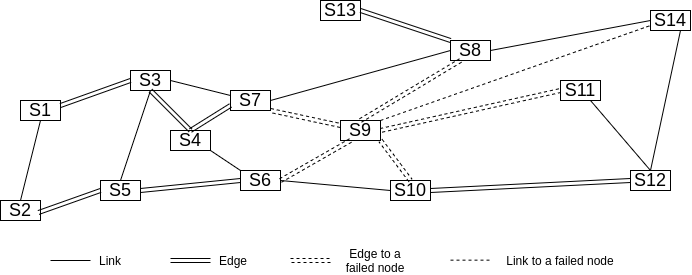
\includegraphics[width=0.8\textwidth]{distributed.png}
    \caption{Codes for neighbouring cells}
    \label{fig:codes}
\end{figure}



The main operations using these locational codes are detailed below:

\begin{enumerate}
    \item \textbf{Computing the code of a cell:} the cell codes are computed when the tree is built. The codes are computed recursively. 
    \item \textbf{Computing the code of sample point:} the code of a sample point $p$ is computed as the integer part of $\frac{p.x-octree.origin.x}{octree.size}\cdot binsize$ expressed in binary notation (and similarly for $p.y$ and $p.z$)
    \item \textbf{Translating the code into a path in the octree:} the code gives a succession of child indices composing the path. For example $(01, 11, 10)$ means the child index 3 followed by 5. 
    \item \textbf{Getting the code of the left neighboring cell:} the code is given by ($cell.xloc - 1$, $cell.yloc-1$, $cell.zloc-1$).
    \item \textbf{Getting the code of the right neighboring cell at level $l$}: the code is given by ($cell.xloc+2^{l}, cell.yloc+2^{l}, cell.zloc+2^{l})$. For leaves, it means computing $(cell.xloc + 1, cell.yloc + 1, cell.zloc+1)$
\end{enumerate}

Here is pseudo-code of octree construction procedure with use of locational codes:

\begin{codebox}\Procname{$\proc{build-octree}(\mathcal{P},r)$}
\li $binsize\leftarrow binary(2^{depth})$
\li \textit{Initialize the octree}: build an empty root cell, set its size to $s$, its origin to $o$, and its level to $depth$

\li \For $p\in\mathcal{P}$ 
\li \Do Compute the codes $xloc$, $yloc$, $zloc$ of $p$ as $xloc=binary(floor(\frac{p.x-octree.origin.x}{octree.size}\cdot bindize))$   \\   \Do(similarly for $yloc$ and $zloc$)\End
\li $cell\leftarrow$ root of the octree
\li $l\leftarrow depth - 1$
\li \While $cell\_depth > 0$ \Do
\li $childbranchbit=1<<l$
\li $x=xloc\&childbranchbit >> l$ (and similarly for $y,z$)
\li $childindex=(x<<2)+(y<<1)+z$
\li \If $cell.child(childindex)$ does not exist \Then \Do
    \li create $cell.child$
    \li $child.size\leftarrow \frac{1}{2}cell.size$
    \li $child.origin.x\leftarrow cell.origin.x + x\cdot child.size$ (similarly for $y,z$) 
    \li $child.depth\leftarrow cell.depth - 1$ 
    \li $child.xloc \leftarrow cell.xloc + (x << child.depth)$ (and similarly for $yloc$ and $zloc$)
    \End\End
    \li $cell = cell.child(childindex)$
    \li $l\leftarrow l - 1$
    \End 
    \li Add $p$ to $cell.points$
\End\End
\end{codebox}

Here:

\begin{enumerate}
    \item[--] \textbf{Line 9:} $childbranchbit$ is a binary integer that in base 2 has a single 1 at position $l+1$ starting from the right. For example $1000$ for level $3$. Then ($xloc&childbrachbit)>>l$) gives either 1 or 0: the next direction to take in the path to the leaf.
    \item[--] \textbf{Line 10:} the child index gives the index (between 0 and 7) corresponding to the child on the path at depth $l$. It is obtained by concatenating the bit at position $l$ in the three codes $xloc$, $yloc$, $zloc$.
    \item[--] \textbf{Line 14:} the origin of the newly created cell is easily deduced from the locational code.
    \item[--] \textbf{Line 16:} to get the code of the child cell, one simply has to add bit $x$ to the code of the parent cell $cell.xloc$ (and similarly for $y$ and $z$).
\end{enumerate}

\begin{lstlisting}[language=C++, caption={Construction of octree}, label={main_1}, basicstyle=\small]
void Octree::build(std::vector<point_t> pts) {
    for(point_t pt: pts) {
        this->add(pt);
    }
}

void Octree::add(point_t point) {
    uint32_t xloc = static_cast<uint32_t>((point.x - this->root->origin.x) 
                    / this->root->size * this->binsize);
    uint32_t yloc = static_cast<uint32_t>((point.y - this->root->origin.y) 
                    / this->root->size * this->binsize);
    uint32_t zloc = static_cast<uint32_t>((point.z - this->root->origin.z) 
                    / this->root->size * this->binsize);

    Cell* cell = this->root;
    uint32_t l = this->root->level - 1;
    while(cell->level !=0) {
        uint32_t child_branch_bit = 1 << l;
        uint32_t x = (xloc & child_branch_bit) >> l;
        uint32_t y = (yloc & child_branch_bit) >> l;
        uint32_t z = (zloc & child_branch_bit) >> l;
        uint32_t idx = (x << 2) + (y << 1) + z;

        if(cell->child[idx] == nullptr) {
            double new_size = cell->size / 2.0;
            point_t new_origin {cell->origin.x + x*new_size,
                                cell->origin.y + y*new_size,
                                cell->origin.z + z*new_size};
            uint32_t new_level = cell->level - 1;

            cell->child[idx] = new Cell(new_origin, new_size, cell->level - 1);
            cell->child[idx]->p = cell;
            cell->child[idx]->xloc = cell->xloc + (x << new_level);
            cell->child[idx]->yloc = cell->yloc + (y << new_level);
            cell->child[idx]->zloc = cell->zloc + (z << new_level);
        }

        cell = cell->child[idx];
        --l;
    }
    cell->data.push_back(point);
}
\end{lstlisting}
\end{comment}


\section{Experiments}


\begin{comment}
As an example of octree use we implement color quantization algorithm. To do this we extend our cells with a reference counter and three color markers. We do not need vector to store data. So the cell looks like:

\begin{lstlisting}[language=C++, caption={Cell for color quantization}, label={main_1}, basicstyle=\small]

class Cell {
public:
    uint32_t xloc;    // Locational code in direction of x-axis
    uint32_t yloc;    // Locational code in direction of z-axis
    uint32_t zloc;    // Locational code in direction of y-axis

    double size;      // Spatial size of the cell in every of x,y,z directions.
    point_t origin;   // Origin
    int level;        // Level of the cell (0 for leaf)
    Cell* p;          // Parent pointer (nullptr for root)
    Cell* child[8];   // Pointers to children

    uint32_t references;
    double red;
    double green;
    double blue;
    cv::Vec3b color;

    Cell(point_t origin, double size, int level) {
        this->origin = origin;
        this->size = size;
        this->level = level;
        this->p = nullptr;
        for(int i=0; i < 8; ++i) {
            this->child[i] = nullptr;
        }

        this->references = 0;
        this->red   = 0.0;
        this->green = 0.0;
        this->blue  = 0.0;
    }

    ~Cell() {
        for(int i=0; i < 8; ++i) {
            if(this->child[i]) {
                delete this->child[i];
                this->child[i] = nullptr;
            }
        }
    }
\end{lstlisting}

Now we insert all colors into the tree each time we found the leaf of the tree we increment the reference count and add the color value to the red, green and blue counters. This will help us to find the colors that are most important. After we inserted all our colors we begin to reduce them. We count all the nodes that have a reference greater than zero (only leafes can have a reference). Now we go into this code:

\begin{codebox}
\li \While number of leafes \ge number of color in palette 
\li \Do search the node, where the sum of the childs references is minimal and reduce it
\End
\end{codebox}

To reduce a node we sum up the color components and reference-counts. 

\begin{lstlisting}[language=C++, caption={Cell reduction}, label={main_1}, basicstyle=\small]
void Cell::reduce() {
    // If this is a leaf - do nothing
    if(this->references != 0) {
        return;
    }

    for(int n = 0; n < 8; ++n) {
        if(this->child[n] != nullptr) {
            this->references += this->child[n]->references;
            this->red += this->child[n]->red;
            this->green += this->child[n]->green;
            this->blue += this->child[n]->blue;

            // Delete the cell. We do not need it anymore
            delete this->child[n];
            this->child[n] = nullptr;
        }
    }
}
\end{lstlisting}

In order to build palette we traverse the tree and if we find a leave we calculate the RGB-components of the node and store them in a palette:


\begin{lstlisting}[language=C++, caption={Build palette}, label={main_1}, basicstyle=\small]
void build_palette(Cell *cell, std::vector<cv::Vec3b> &palette) {
    for(int n=0; n < 8; ++n) {
        if(cell->child[n] != nullptr){
            if(cell->child[n]->references == 0) {
                build_palette(cell->child[n], palette);
            } else {
                cell->color(2) = 
                    static_cast<uint8_t>(cell->child[n]->red 
                    / cell->child[n]->references);
                cell->color(0) = 
                    static_cast<uint8_t>(cell->child[n]->green 
                    / cell->child[n]->references);
                cell->color(1) 
                    = static_cast<uint8_t>( cell->child[n]->blue 
                    / cell->child[n]->references);
                palette.push_back(cell->color);
            }
        }
    }
}
\end{lstlisting}

In order to run node reduction we have to find all the nodes that have only leaf-children:

\begin{lstlisting}[language=C++, caption={Find nodes with only leaf-children}, label={main_1}, basicstyle=\small]
void get_over_leafs(Cell *cell, std::vector<Cell*> &leafs) {
    bool is_overleaf = true;
    for(int n=0; n < 8; ++n) {
        if((cell->child[n] != nullptr) 
            && (cell->child[n]->references == 0)) {
            get_over_leafs(cell->child[n], leafs);
            is_overleaf = false;
        };
    }
    if(is_overleaf) {
        leafs.push_back(cell);
    }
}
\end{lstlisting}

So, to build the color palette we first populate octree with all available pixel data. Then we run node reduction until the number of leafs is not equal to number of desired color in the palette. To get colors of palette we have to divide each color component in leafs nodes to number of references. Example of quantization of images with this algorithm are presented in figures \ref{fig:rainbow} and \ref{fig:baboon}.

\begin{figure}[ht!]
    \centering
    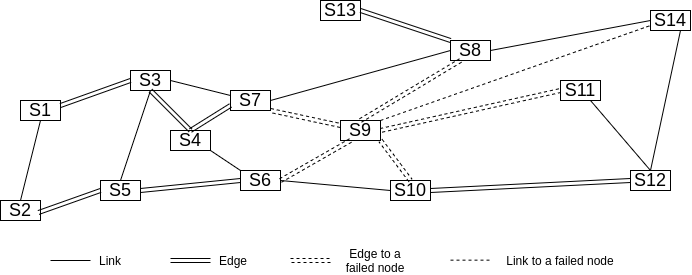
\includegraphics[width=0.45\textwidth]{distributed.png}
    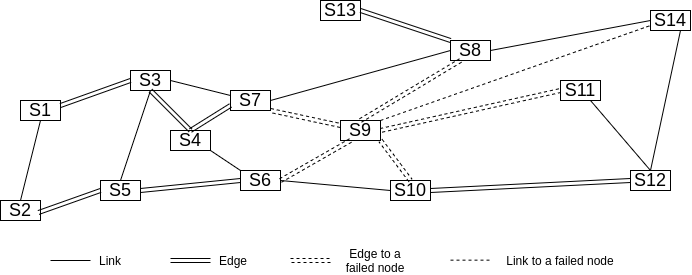
\includegraphics[width=0.45\textwidth]{distributed.png}
    \caption{Quantization of a rainbow image with number of colors = 256}
    \label{fig:rainbow}
\end{figure}

\begin{figure}[ht!]
    \centering
    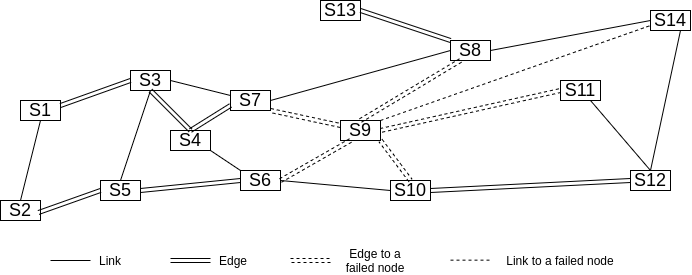
\includegraphics[width=0.45\textwidth]{distributed.png}
    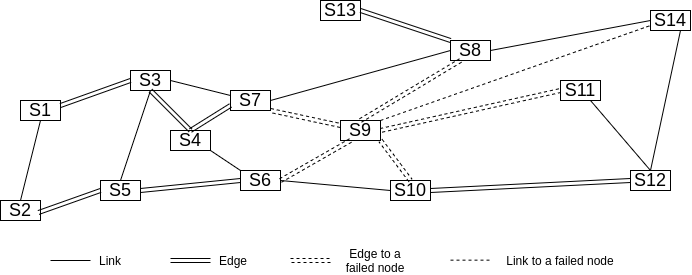
\includegraphics[width=0.45\textwidth]{distributed.png}
    \caption{Quantization of a baboon image with number of colors = 20}
    \label{fig:baboon}
\end{figure}
\end{comment}

\section{Conclusions}

We deserve an A. 



\printbibliography
\newpage
\appendix
\section{Code}

\begin{lstlisting}[language=python, caption={Color quantization program}, label={main_1}, basicstyle=\small]
import os
import sys

id_table = dict()

class Node(object):
    def __init__(self, id, links):
        self.id = id
        self.ports = {i: nb_id for i, nb_id in enumerate(links)}
        self.edges = []

        # State variables
        self.coord_so_far = None
        self.port_to_coord = None
        self.status = 'idle'
        self.recd_reply = {}

    def init_reconfig(self):
        for port in self.ports.values():
            self.get_node(port).reconfig([self.id], self.id)

    def get_node(self, node_id):
        return id_table[node_id]

    def no_contention(self, from_id):
        print('Node {} recieved no_contention({})'.format(self.id, from_id))
        self.recd_reply[from_id] = 'no_contention'
        self.process(from_id)

    def accepted(self, from_id):
        print('Node {} recieved accepted({})'.format(self.id, from_id))
        self.recd_reply[from_id] = 'accepted'
        self.process(from_id)

    def process(self, from_id):
        from_port = self.port_to(from_id)
        if from_id in self.set_of_ports().difference([from_port]):
            if 'accepted' in self.recd_reply.values():
                self.get_node(self.ports[self.port_to_coord]).accepted(self.id)
                if self.port_to_coord not in self.get_port():
                    self.assign_edge(self.port_to_coord)
            else:
                if (self.port_to_coord not in self.get_port()) and len(self.set_of_ports().difference([self.port_to_coord]).intersection(self.get_port()))!=0:
                    self.get_node(self.ports[self.port_to_coord]).accepted(self.id)
                    self.assign_edge(self.port_to_coord)
        else:
            self.get_node(self.ports[self.port_to_coord]).no_contention(self.id)

    def reconfig(self, node_list, frag_id):
        print('Node {} recieved reconfig({}, {})'.format(self.id, node_list, frag_id))
        sender_id = node_list[-1]
        if self.status == 'idle':
            if len(self.ports) == 1:
                self.get_node(sender_id).no_contention(self.id)
            self.coord_so_far = frag_id
            self.status = 'wait'
            self.port_to_coord = self.port_to(sender_id)
            for port in set(self.ports.keys()).difference([self.port_to(sender_id)]):
                self.get_node(self.ports[port]).reconfig(node_list + [self.id], frag_id)
        elif self.status == 'wait':
            e = self.port_to(sender_id)
            if (frag_id == self.coord_so_far) and (e not in self.get_port()):
                self.get_node(self.ports[e]).no_contention(self.id)
                return
            if self.id in node_list:
                self.get_node(self.ports[e]).no_contention(self.id)
                return
        # Resolve contention
        if (self.coord_so_far > frag_id) or ((self.coord_so_far == frag_id) and (self.id > sender_id)):
            self.get_node(sender_id).stop(self.coord_so_far, from_id=self.id)
        else:
            self.coord_so_far = frag_id
            self.get_node(self.ports[self.port_to_coord]).stop(frag_id, from_id=self.id)
            self.port_to_coord = self.port_to(sender_id)

    def stop(self, frag_id, from_id):
        print('Node {} recieved stop({}, {})'.format(self.id, frag_id, from_id))
        p = self.port_to(from_id)
        if frag_id > self.coord_so_far:
            self.coord_so_far = frag_id
            self.get_node(self.ports[self.port_to_coord]).stop(frag_id, from_id=self.id)
            self.port_to_coord = p
        if frag_id == self.coord_so_far:
            if self.port_to_coord not in self.get_port():
                self.get_node(self.ports[self.port_to_coord]).no_contention(self.id)
                self.recd_reply[self.port_to_coord] = 'no_contention'
            else:
                self.get_node(self.ports[self.port_to_coord])
            self.port_to_coord = p
        if frag_id < self.coord_so_far:
            self.get_node(self.ports[p]).stop(frag_id, from_id=self.id)

    def port_to(self, node_id):
        for port_idx, cur_id in self.ports.items():
            if cur_id == node_id:
                return port_idx
        return None

    def set_of_ports(self):
        return set(self.ports.keys())

    def assign_edge(self, port_id):
        self.edges.append(port_id)

    def get_port(self):
        return self.edges

if __name__ == '__main__':
    id_table.update({1: Node(1, links=[3, 2]),
                2: Node(2, links=[1, 5]),
                3: Node(3, links=[1, 5, 4, 7]),
                4: Node(4, links=[3, 7, 6]),
                5: Node(5, links=[2, 3, 6]),
                6: Node(6, links=[4, 5]),
                7: Node(7, links=[3, 4])})
    id_table[1].init_reconfig()
\end{lstlisting}


\end{document}
